\subsubsection{UC18 - Eliminazione dizionario dati}\label{UC18}

\begin{figure}[H]
  \centering
  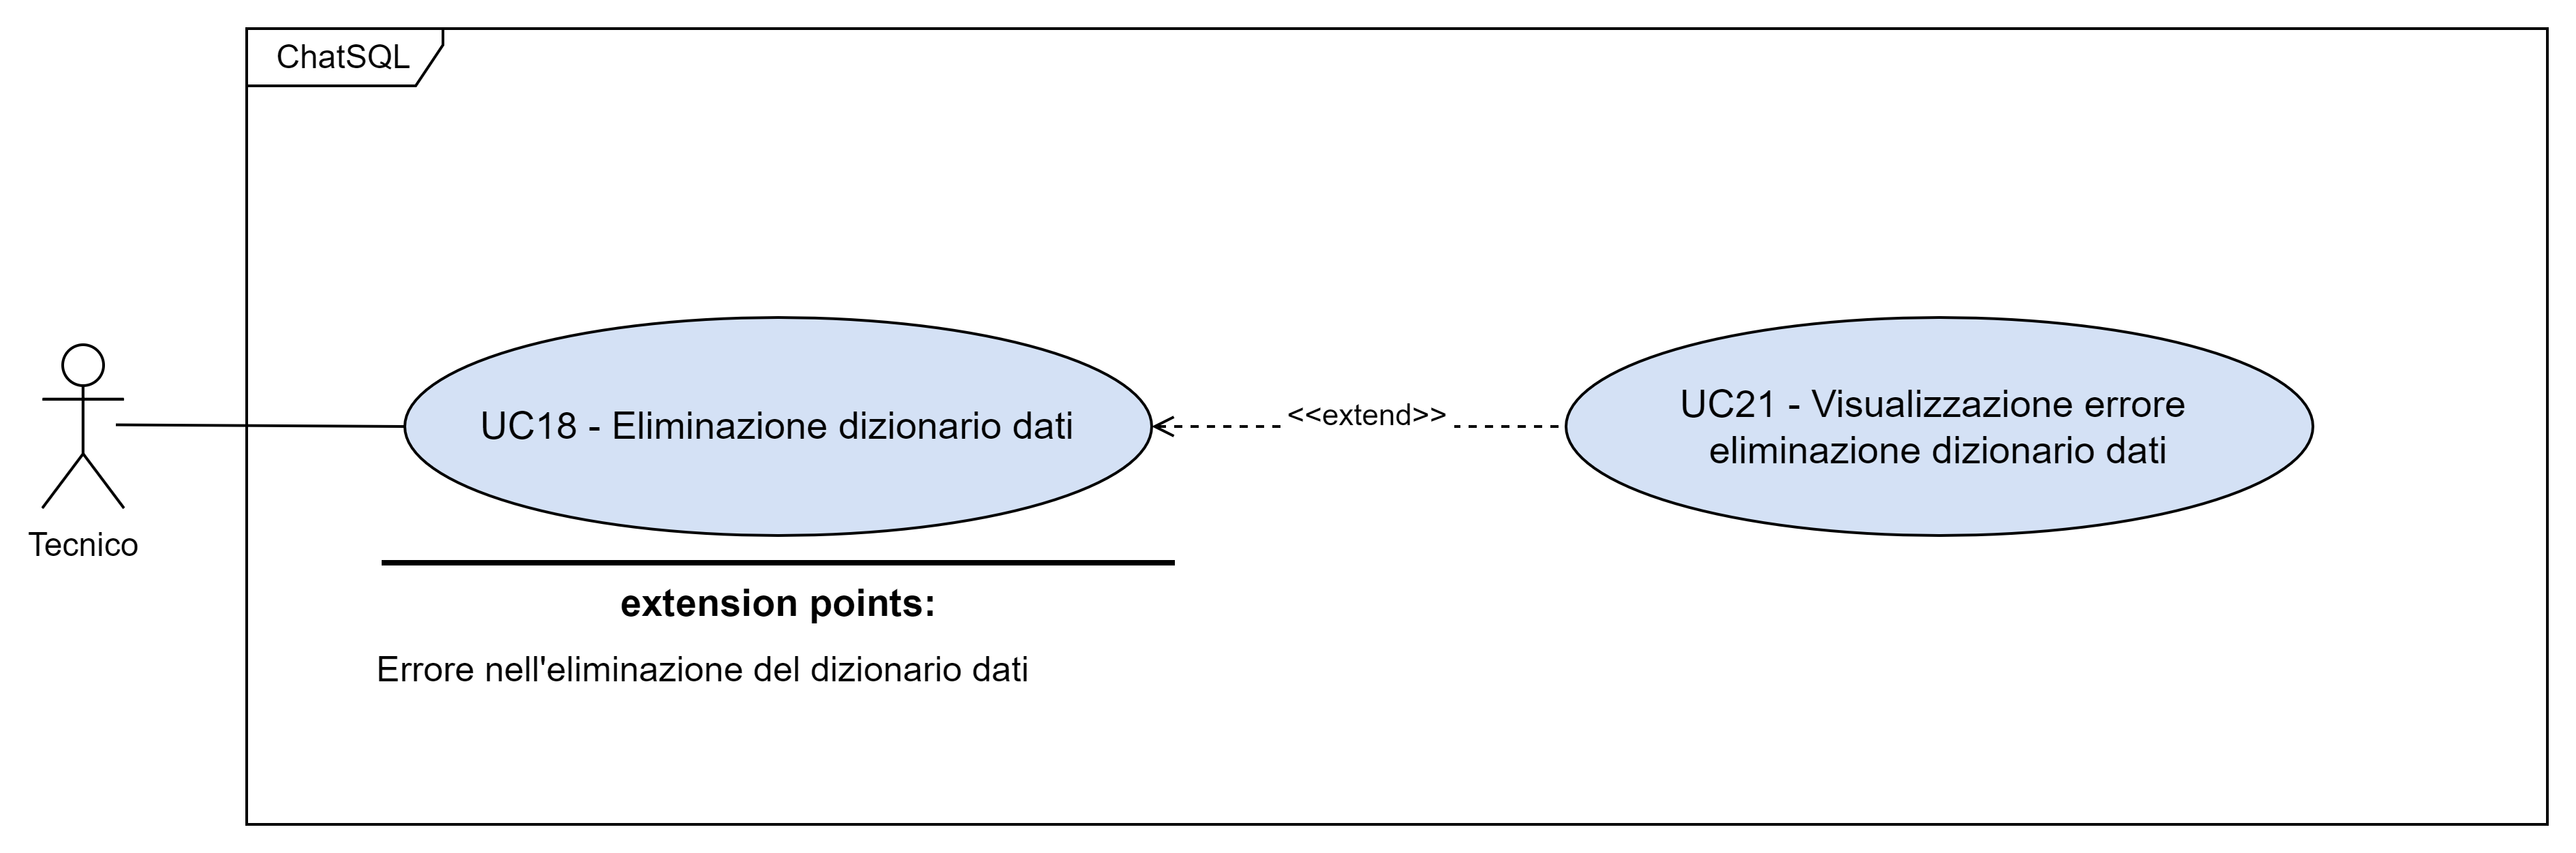
\includegraphics[width=0.95\textwidth]{assets/uc18.png}
  \caption{UC18}
\end{figure}

\paragraph*{Descrizione}
Il Tecnico elimina un \glossario{dizionario dati} dall'applicazione.

\paragraph*{Attori principali}
Tecnico

\paragraph*{Precondizioni}
\begin{itemize}
  \item Il sistema è attivo e funzionante;
  \item Il Tecnico ha effettuato l'autenticazione (\hyperref[UC1]{UC1});
  \item Il Tecnico ha visualizzato la lista dei \glossario{dizionari dati} (\hyperref[UC9]{UC9});
  \item Il Tecnico ha individuato il dizionario da eliminare (\hyperref[UC9.1]{UC9.1}).
\end{itemize}

\paragraph*{Postcondizioni}
\begin{itemize}
  \item Il \glossario{dizionario dati} è stato rimosso con successo;
  \item Il dizionario dati non è più disponibile per gli utenti dell'applicazione.
\end{itemize}

\paragraph*{Trigger}
Il Tecnico vuole eliminare un \glossario{dizionario dati}.

\paragraph*{Scenario principale}
\begin{enumerate}
  \item Il Tecnico tenta di eliminare un \glossario{dizionario dati};
  \item Il sistema richiede una conferma per procedere con l'eliminazione;
  \item Il Tecnico conferma la decisione;
  \item Il dizionario dati viene rimosso dalla lista dei dizionari presenti nel sistema.  
\end{enumerate}

\paragraph*{Scenario alternativo}
\begin{enumerate}
  \item Il sistema riscontra un errore nel tentativo di eliminare il \glossario{dizionario dati} (\hyperref[UC21]{UC21});
  \item Viene restituito un messaggio con i dettagli riguardanti l'errore.
\end{enumerate}

\paragraph*{Estensioni}
\begin{itemize}
  \item Visualizzazione errore eliminazione dizionario dati (\hyperref[UC21]{UC21}):
  \begin{itemize}
    \item Extension point: Errore nell'eliminazione del dizionario dati.
  \end{itemize}
\end{itemize}